\documentclass[11pt]{beamer}
\usetheme{Warsaw}
\usepackage[utf8]{inputenc}
\usepackage[german]{babel}
\usepackage[T1]{fontenc}
\usepackage{amsmath}
\usepackage{amsfonts}
\usepackage{amssymb}
\usepackage{graphicx}
\author{Stefan Zaufl, Christian Brändle, Dominik Schörkhuber}
\title{3D Vision UE}
%\setbeamercovered{transparent} 
%\setbeamertemplate{navigation symbols}{} 
%\logo{} 
%\institute{} 
%\date{} 
%\subject{} 
\begin{document}

\begin{frame}
\titlepage
\end{frame}

%\begin{frame}
%\tableofcontents
%\end{frame}

\begin{frame}{Budha}
\center
	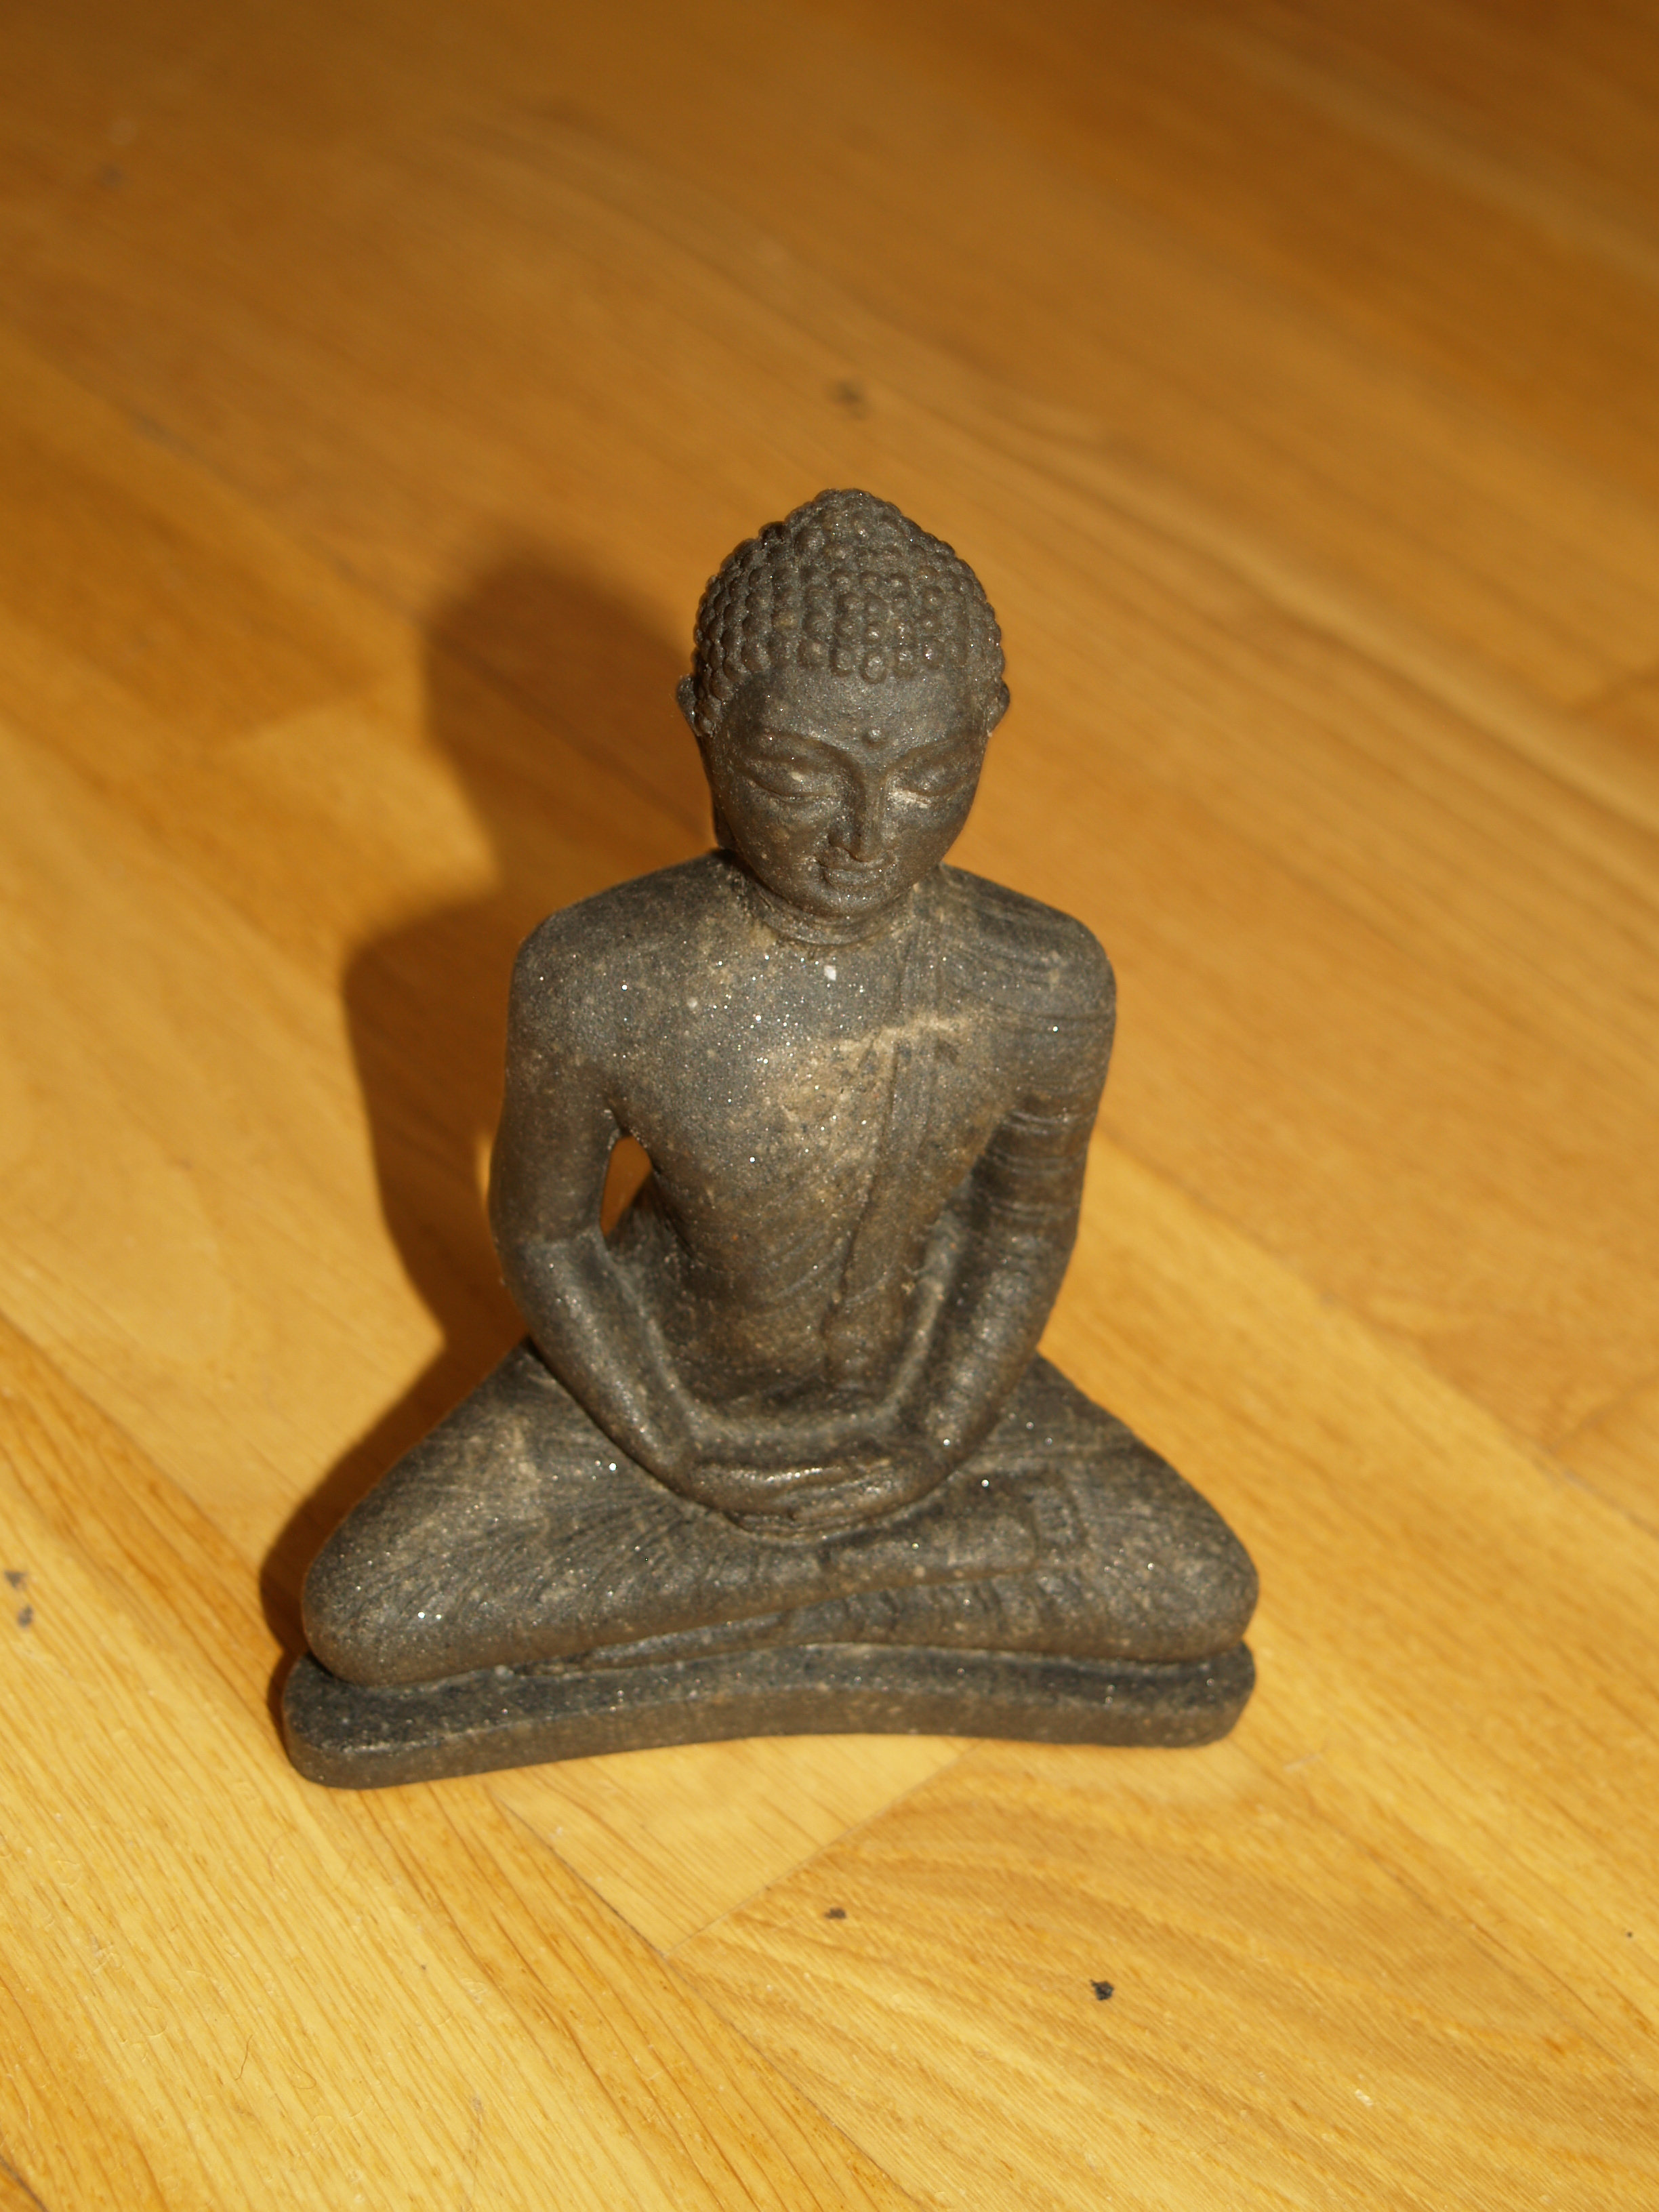
\includegraphics[width=3cm]{images/budha/Budha_original.jpg}
	\begin{block}{Objektbeschreibung}
		\begin{itemize}
			\item rauhe Oberfläche
			\item gesprenkelte Texturierung
			\item viele feine Details
			\item matt \& dunkel
		\end{itemize}
	\end{block}

\end{frame}

\begin{frame}{Finales Modell - Budha}
\center
	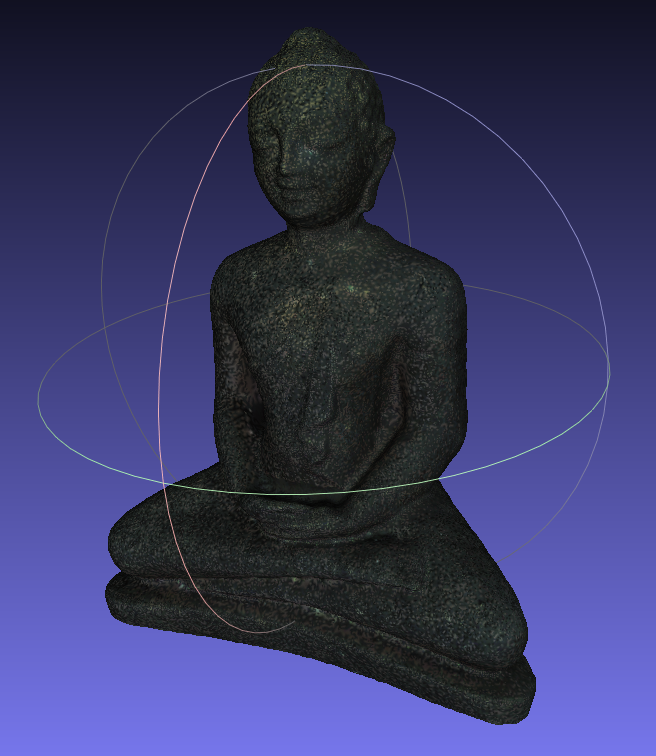
\includegraphics[height=4.3cm]{images/budha/Budha_3DScan_Untextured_2.png}
	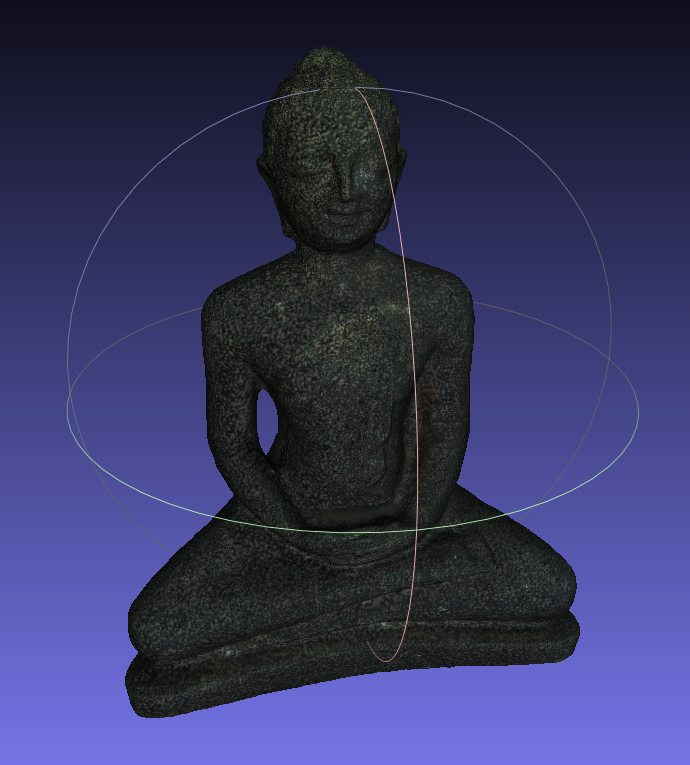
\includegraphics[height=4.3cm]{images/budha/Budha_3DScan_Untextured.png}
	\begin{block}{Objektbeschreibung}
		\begin{itemize}
			\item Global, Manuell Registriert, Vereinigt
			\item Meshdoctor zur Analyse
			\item manuelle Entfernung von Meshfehlern mit anschließendem Schließen
			\item Smoothing
		\end{itemize}
	\end{block}
\end{frame}

\begin{frame}{123d Catch - Budha}
\center
	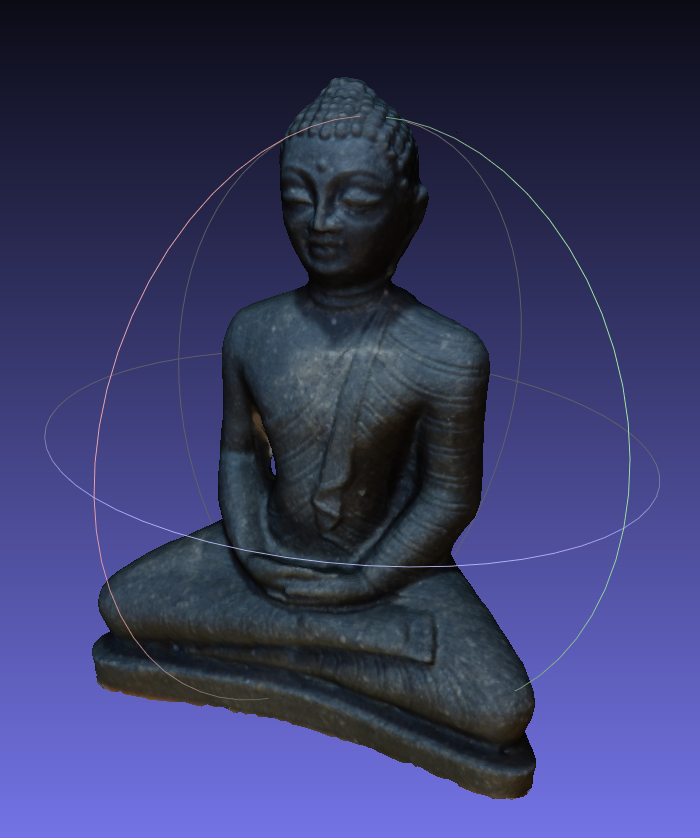
\includegraphics[height=4.5cm]{images/budha/Budha_SfM_Textured.png}
	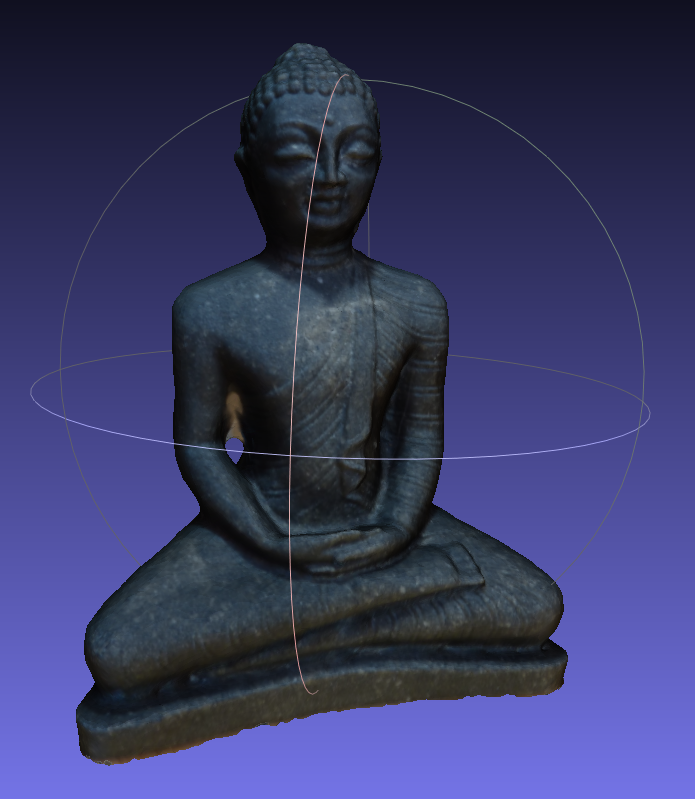
\includegraphics[height=4.5cm]{images/budha/Budha_SfM_Textured_2.png}
	\begin{block}{Objektbeschreibung}
		\begin{itemize}
			\item Viel Textur und Geometrie -> gute Features
			\item Nachbearbeitung: Trennen der Figur vom Untergrund \& Loch schließen
		\end{itemize}
	\end{block}
\end{frame}

\begin{frame}{Evaluierung - Budha}

	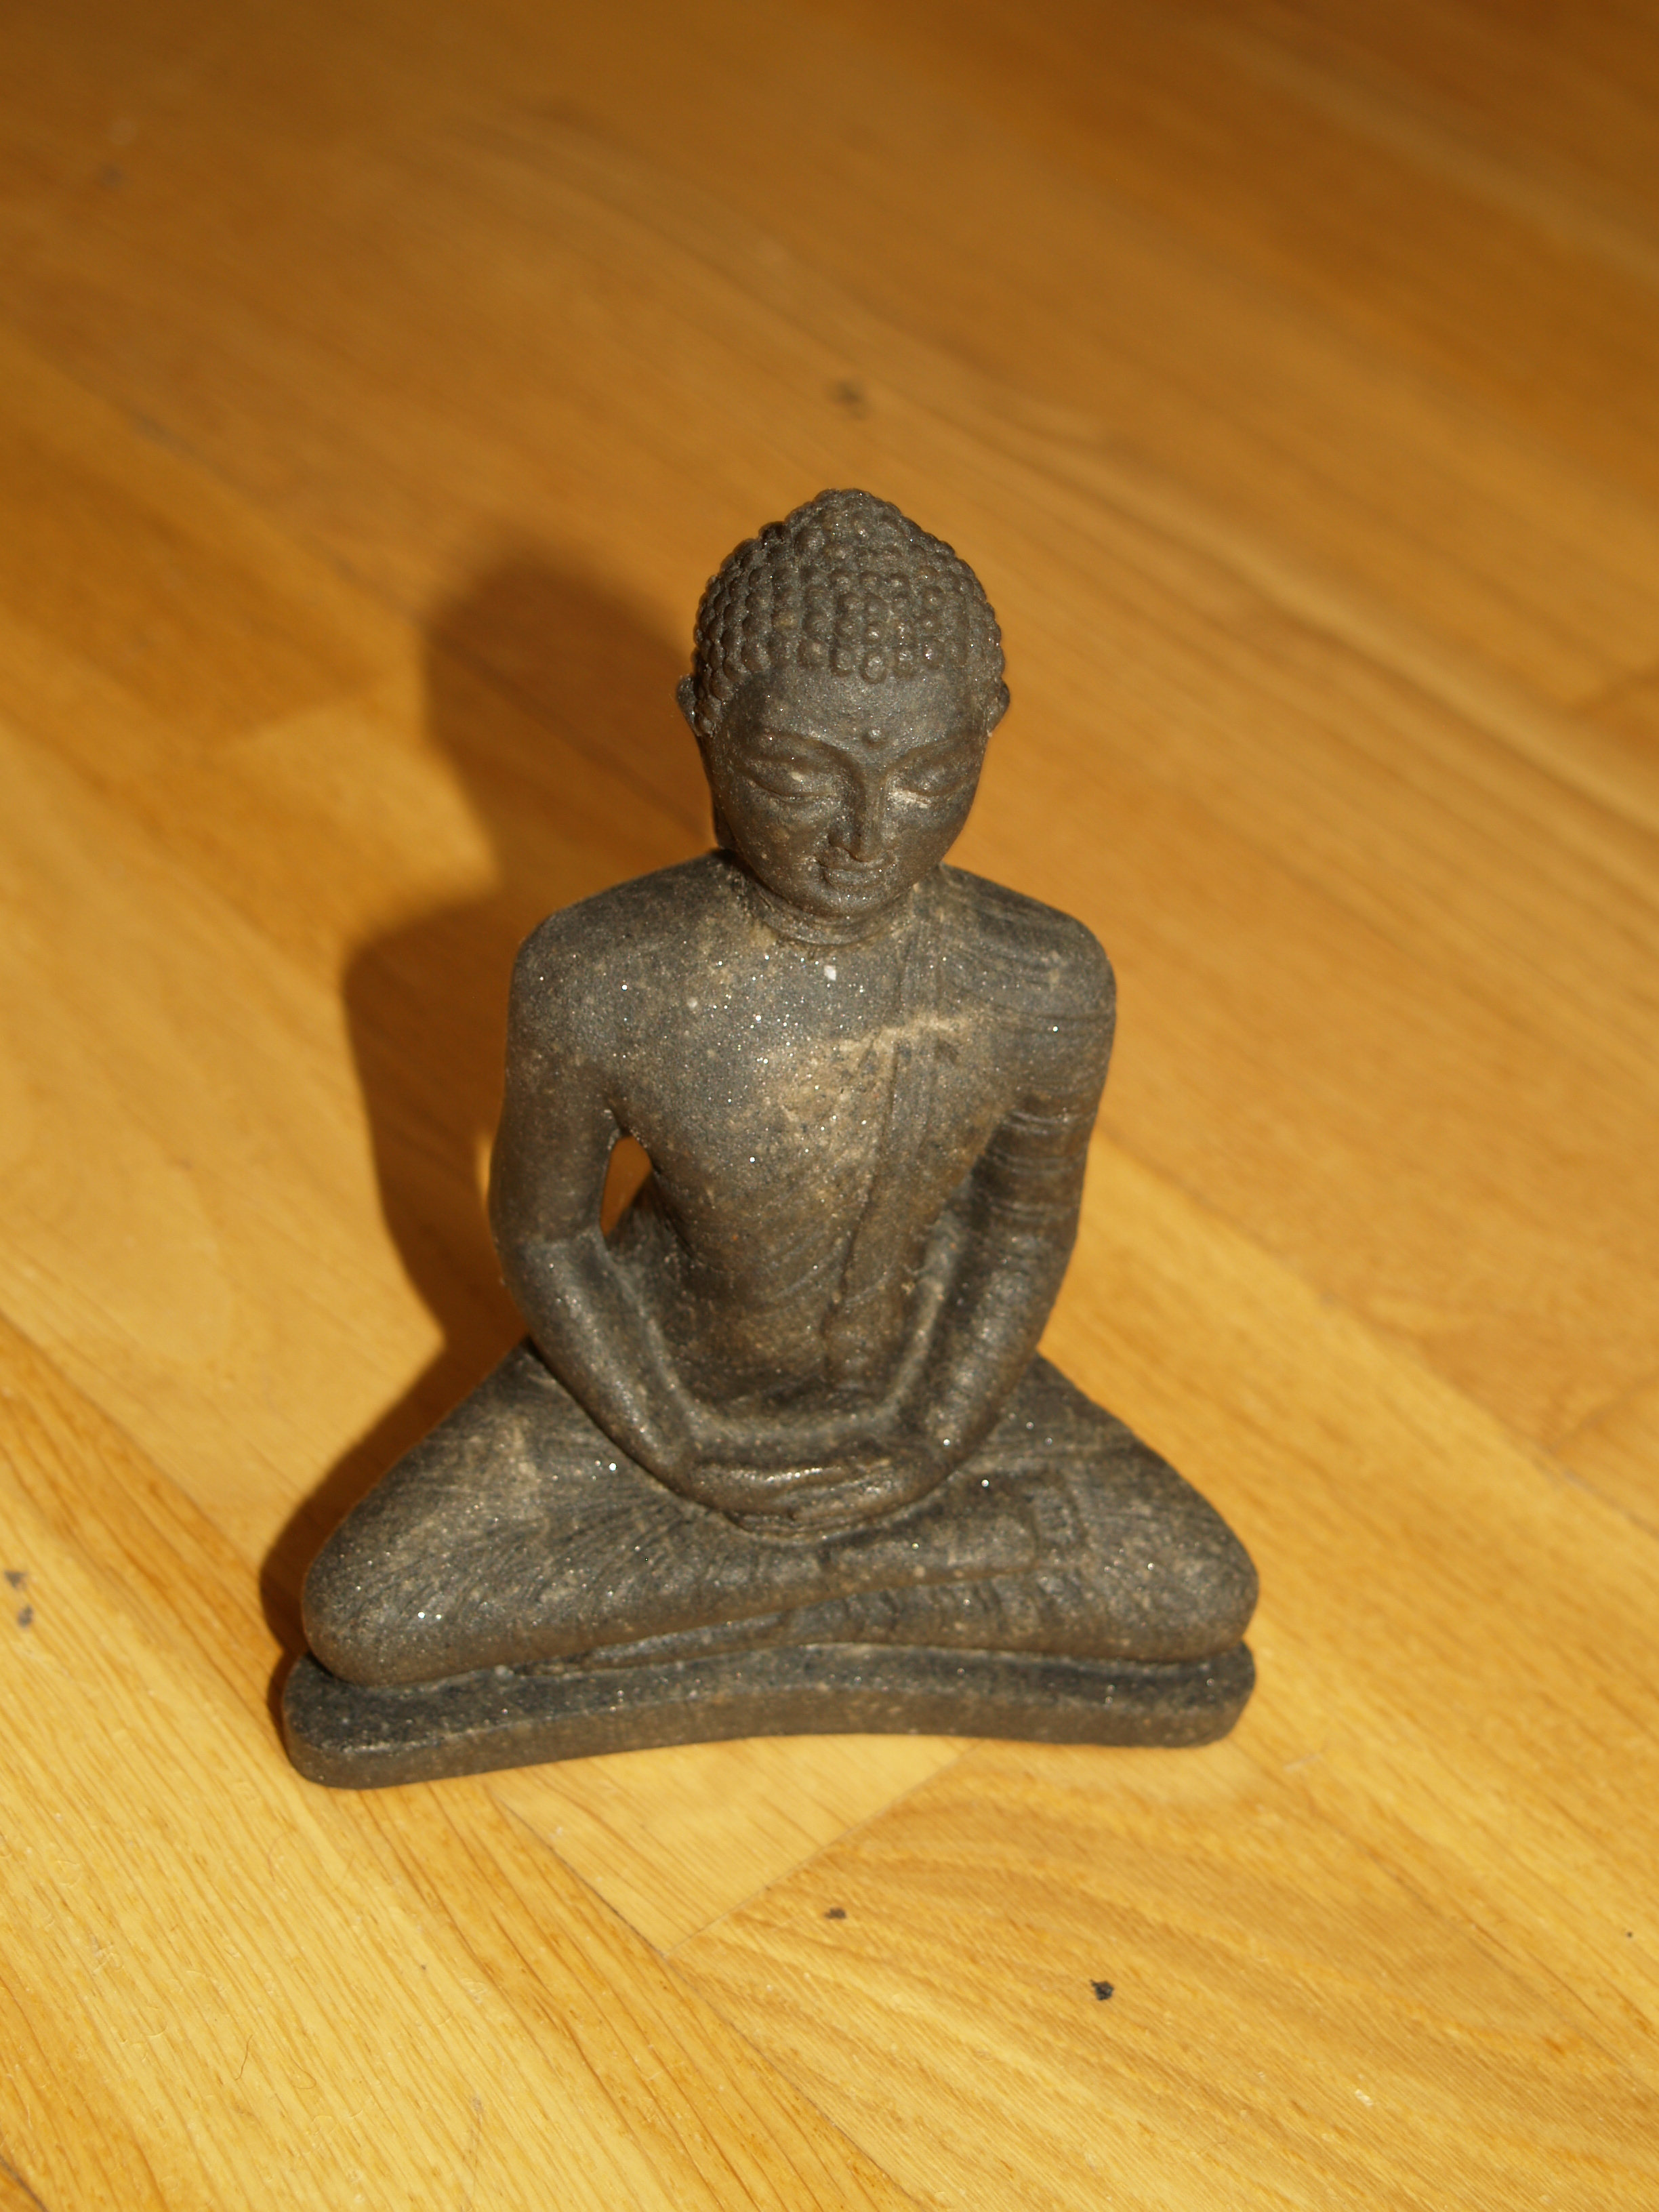
\includegraphics[height=2.5cm]{images/budha/Budha_original.jpg}
	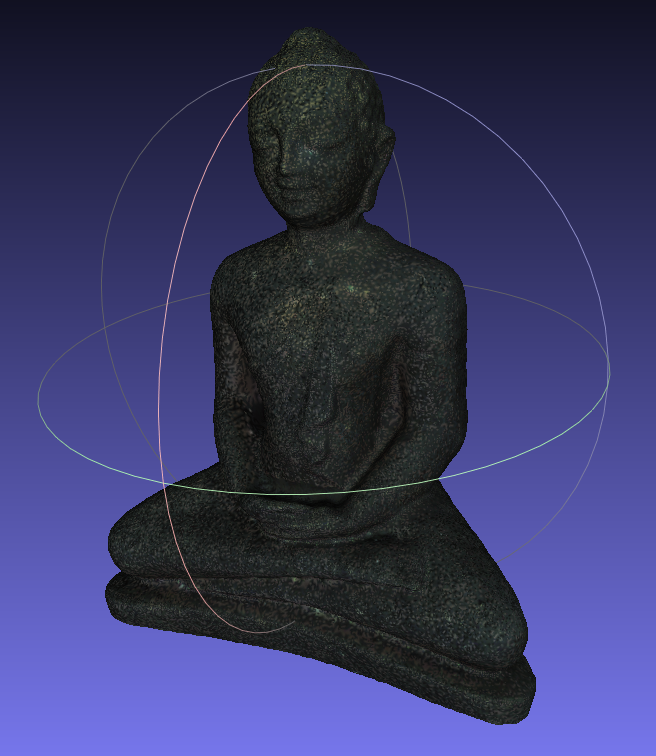
\includegraphics[height=2.5cm]{images/budha/Budha_3DScan_Untextured_2.png}
	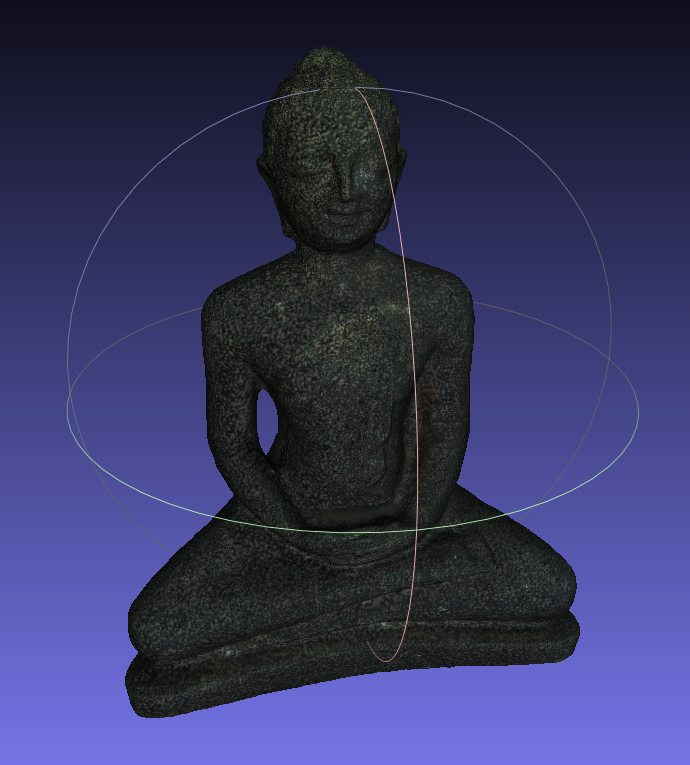
\includegraphics[height=2.5cm]{images/budha/Budha_3DScan_Untextured.png}
	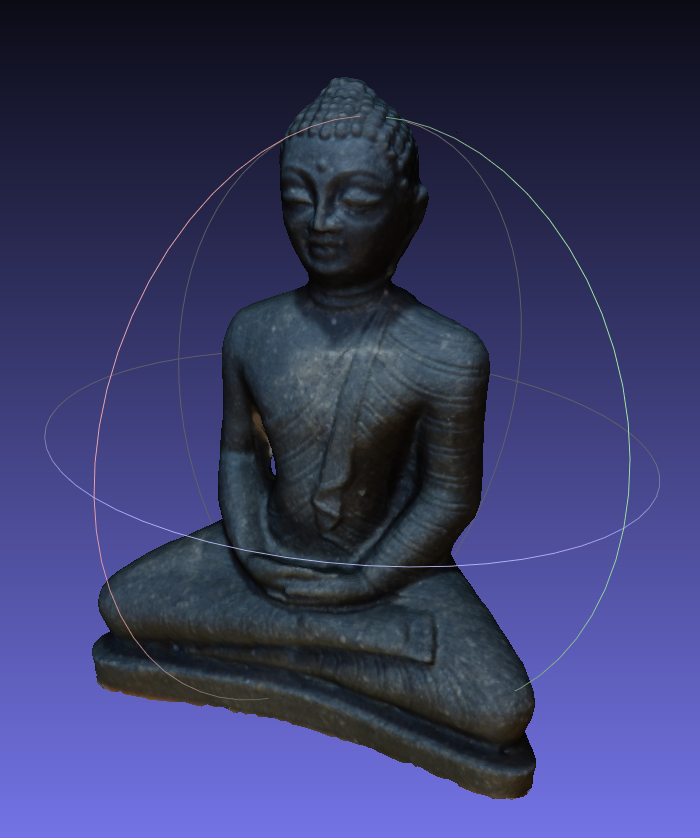
\includegraphics[height=2.5cm]{images/budha/Budha_SfM_Textured.png}
	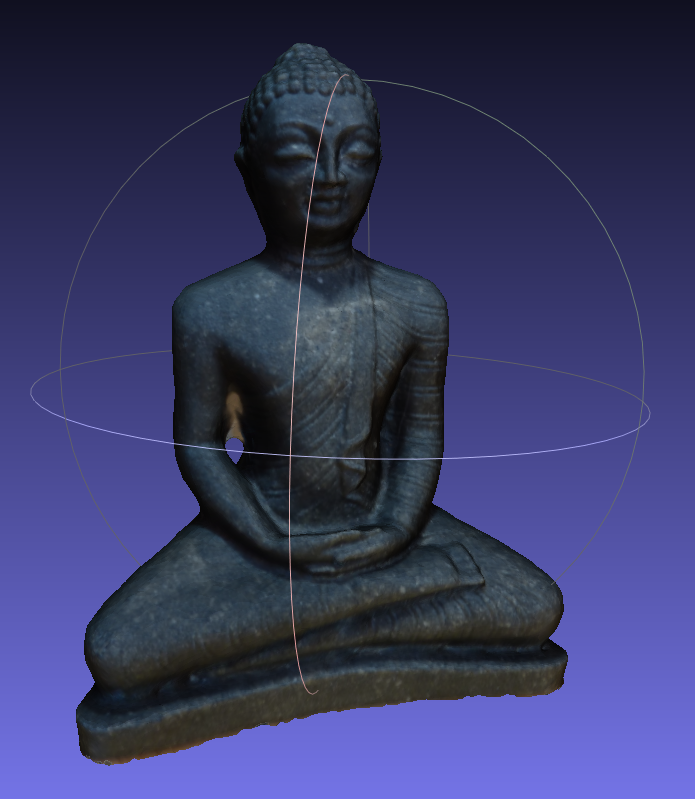
\includegraphics[height=2.5cm]{images/budha/Budha_SfM_Textured_2.png}
	
	\begin{block}{Messpunkte}
		\begin{itemize}
			\item Fußpunkt
			\item Haaransatz
		\end{itemize}
	\end{block}
	\begin{block}{Messfehler}
		Abweichung von $5 \%$ im Volumen
	\end{block}
\end{frame}


\begin{frame}{Sparschwein}
\center
	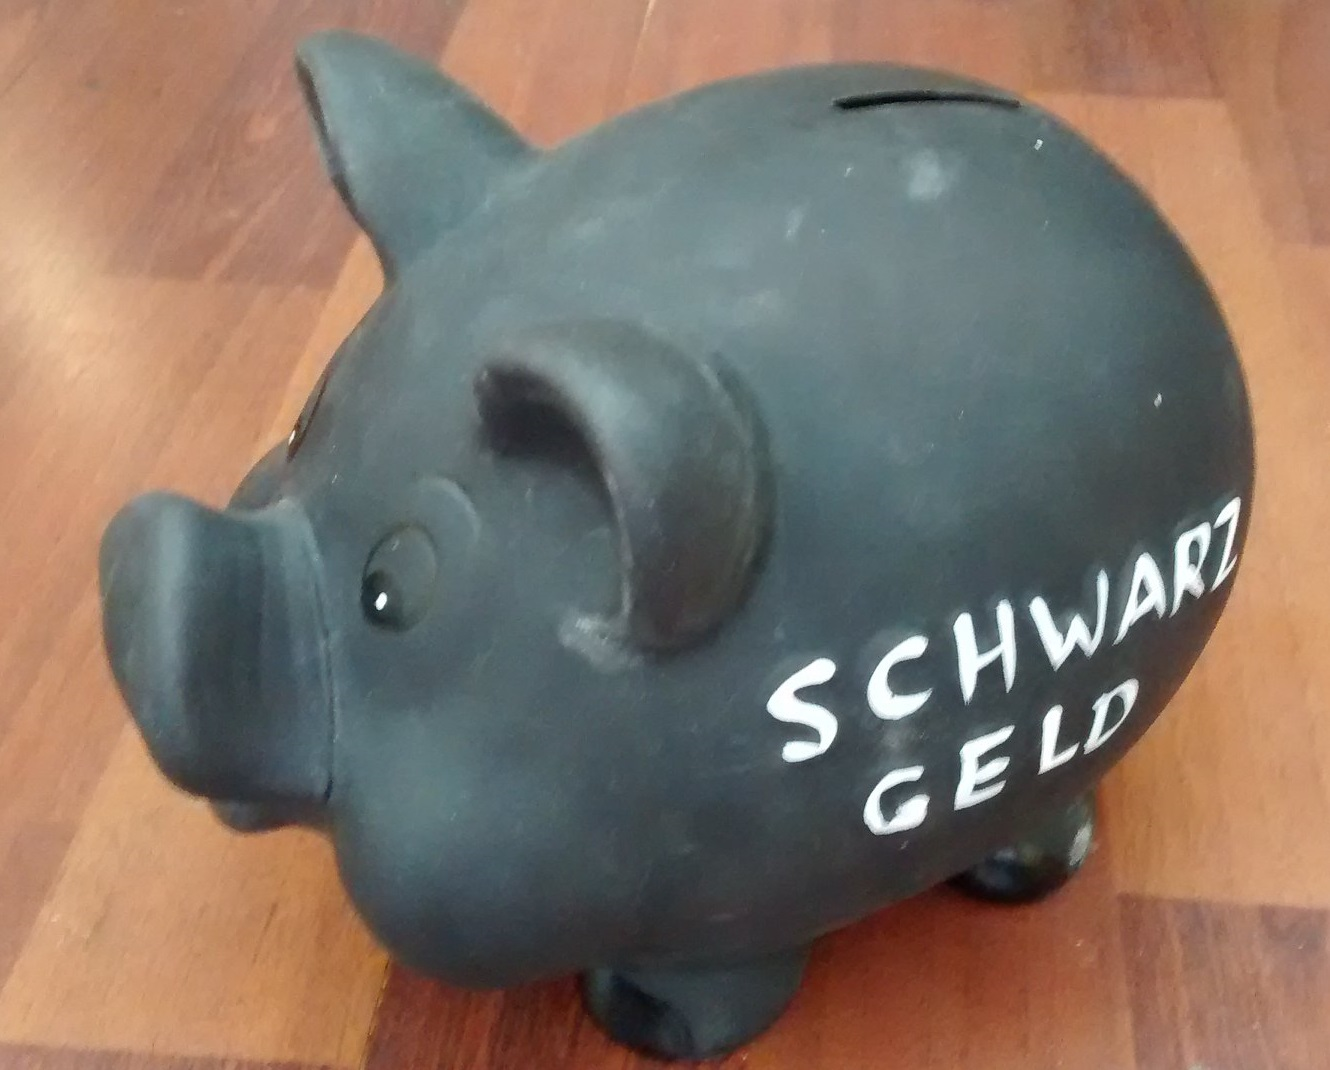
\includegraphics[width=5cm]{images/sparschwein/photo.jpg}
	\begin{block}{}
		\begin{itemize}
			\item Einfache Geometrie
			\item Sehr dunkel -> Laser Intensität
			\item Reflektierende Teile
		\end{itemize}
	\end{block}

\end{frame}

\begin{frame}{Finales Modell - Sparschwein}
\center
	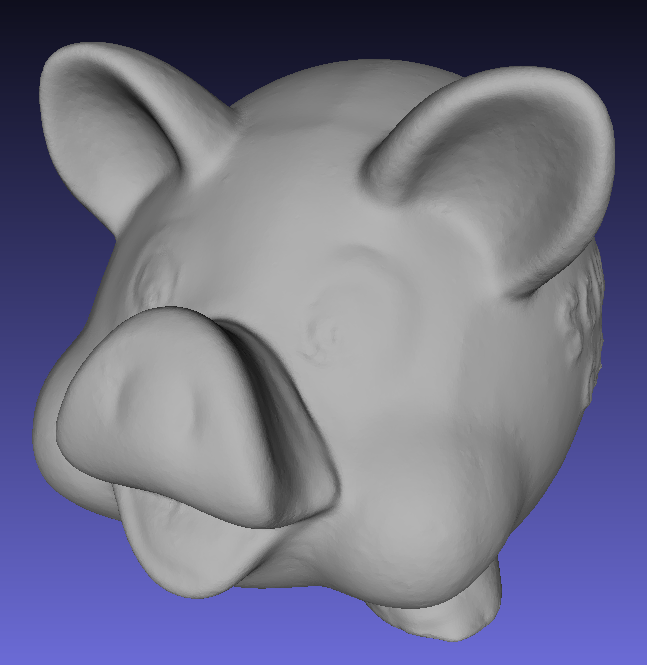
\includegraphics[height=5cm]{images/sparschwein/final2}
	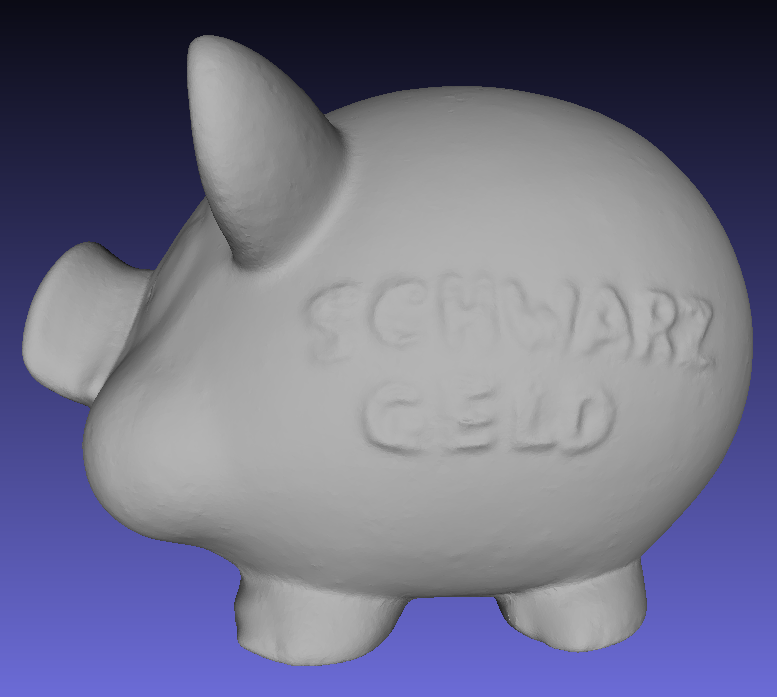
\includegraphics[height=5cm]{images/sparschwein/final3}
	\begin{block}{}
		\begin{itemize}
			\item Global, Manuell Registriert, Vereinigt
			\item Meshdoctor
			\item Fehlende Geometrie an den Zehen wiederhergestellt
			\item Sanding
		\end{itemize}
	\end{block}
\end{frame}

\begin{frame}{123d Catch - Sparschwein}
\center
	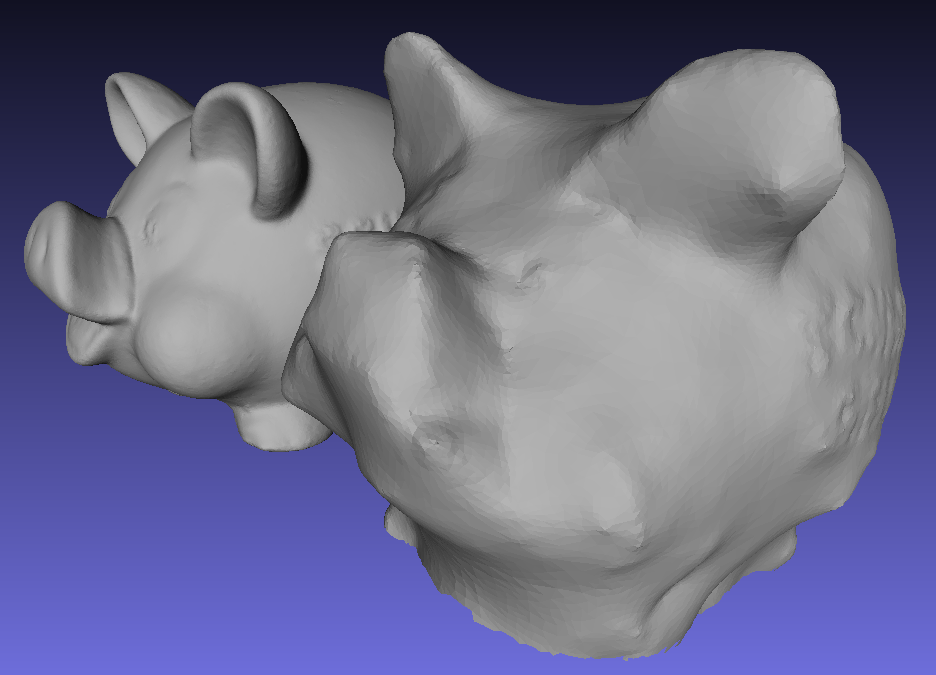
\includegraphics[width=10cm]{images/sparschwein/123d_Vergleich}
	\begin{block}{}
		\begin{itemize}
			\item Wenig Textur -> wenig Features :(
			\item Erst durch manuelle Registrierung brauchbar
		\end{itemize}
	\end{block}
\end{frame}

\begin{frame}{Evaluierung - Sparschwein}
	\begin{block}{Messpunkte}
		\begin{itemize}
			\item Nasenbreite
			\item Ohrenbreiten
			\item Münzschlitzlänge
			\item Münzauswurf Durchmesser
			\item Schriftgröße
		\end{itemize}
	\end{block}
	\begin{block}{}
		Abweichung von $\pm1$mm
	\end{block}
\end{frame}



\end{document}